\documentclass[tikz, border=2pt]{standalone}
\usepackage{amsmath}

\begin{document}
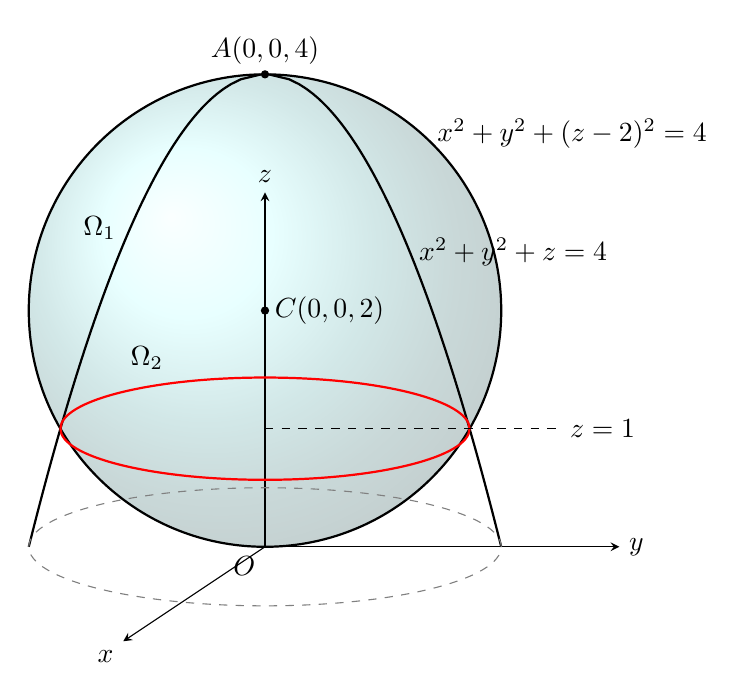
\begin{tikzpicture}[scale=1.5, >=stealth]
    % 1. 绘制球体（半透明 shading 和轮廓）
    \shade[ball color=cyan!40, opacity=0.3] (0,2) circle (2);
    \draw[thick] (0,2) circle (2);
    
    % 2. 绘制坐标轴
    \draw[->] (0,0) -- (3,0) node[right] {$y$};
    \draw[->] (0,0) -- (0,3) node[above] {$z$};
    \draw[->] (0,0) -- (-1.2,-0.8) node[below left] {$x$};
    
    % 3. 绘制抛物面轮廓（两条抛物线，对应 y=0 截面）
    \draw[thick, domain=0:4, samples=100] plot ({sqrt(4-\x)}, \x);
    \draw[thick, domain=0:4, samples=100] plot ({-sqrt(4-\x)}, \x);
    
    % 4. 绘制底面圆（z=0 处，抛物面与 xy 平面交线）
    \draw[dashed, gray] (0,0) ellipse (2 and 0.5);
    
    % 5. 绘制交线圆（z=1 处，球面与抛物面交线）
    \draw[thick, red] (0,1) ellipse (1.732 and 0.433);
    \draw[dashed] (0,1) -- (2.5,1) node[right] {$z=1$};
    
    % 6. 标注关键点
    \fill (0,2) circle (1pt) node[right] {$C(0,0,2)$};
    \fill (0,4) circle (1pt) node[above] {$A(0,0,4)$};
    \node[below left] at (0,0) {$O$};
    
    % 7. 标注两部分区域
    \node at (-1.4,2.7) {$\Omega_1$};
    \node at (-1,1.6) {$\Omega_2$};
    
    % 8. 球体方程
    \node at (2.1,2.5) {$x^2+y^2+z=4$};
    \node at (2.6,3.5) {$x^2+y^2+(z-2)^2=4$};
\end{tikzpicture}
\end{document}